% ─── Slide: PTQ plateau ───────────────────────────────────────────────────────
\begin{frame}[shrink=20]{Pure PTQ Hits a Plateau — a Different Tool Is Needed}
  \begin{columns}[T]
    \begin{column}{0.50\textwidth}
      After all PTQ improvements (v2 through v5):
      \begin{itemize}
        \item Best $\adcppl \approx 27.5\text{--}28.5$ across all INT4 variants
        \item Adding more calibration samples / stochastic propagation / Hadamard
              gives $< 0.5$ PPL gain
        \item \textbf{Root cause:} 4-bit weight quantisation introduces
              systematic residual error that transform calibration
              cannot recover — transforms redistribute information,
              but cannot add it back after INT4 rounding
      \end{itemize}

      \vspace{0.15em}
      \begin{alertblock}{Key realisation}
        We need a \textbf{post-hoc correction} that can learn to model
        the ADC residual \emph{after} quantisation, without
        re-training the frozen PTQ checkpoint.
      \end{alertblock}
    \end{column}
    \begin{column}{0.46\textwidth}
      % plot_ptq_plateau.pdf
      \iftrue
        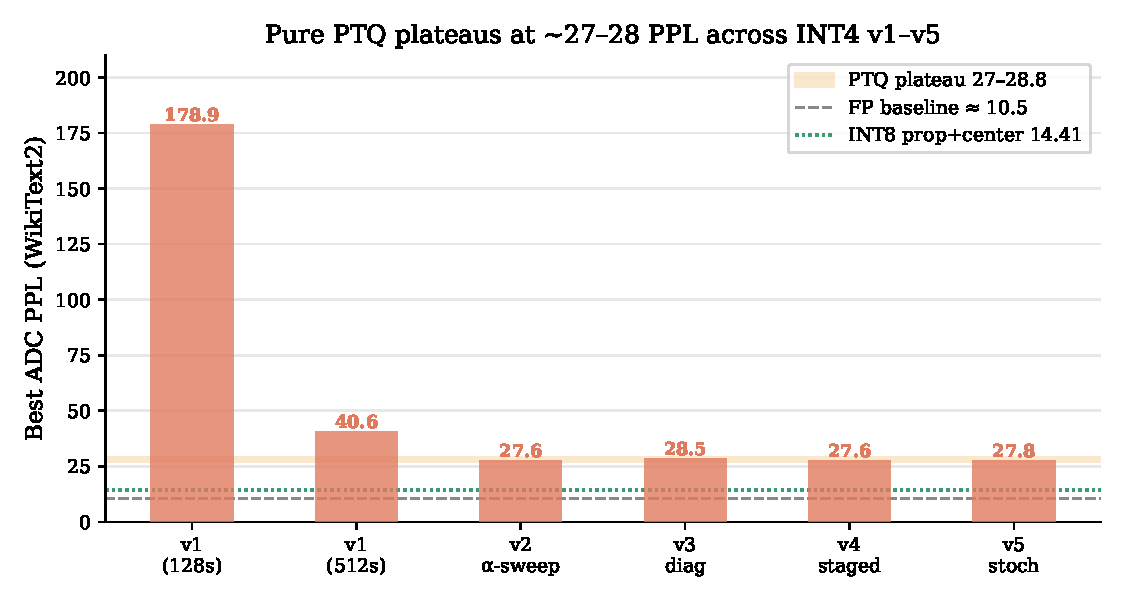
\includegraphics[width=\linewidth]{figs/plot_ptq_plateau.pdf}
      \else
        \figplaceholder[0.65\textheight]{Scatter / step plot: all INT4 PTQ variants (v1--v5)
          on x-axis, ADC PPL on y-axis.
          Color by version (v1=128s, v2=1024s alpha-sweep, v3=diag, v4=staged, v5=stoch).
          Draw a horizontal band at 27--28.5 labeled ``PTQ plateau''.
          Draw FP baseline at 10.5 and INT8 prop+center at 14.41 as dashed lines.}
      \fi
    \end{column}
  \end{columns}
\end{frame}
